\documentclass[11pt,a4paper]{article}

% Packages
\usepackage[utf8]{inputenc}
\usepackage[T1]{fontenc}
\usepackage{amsmath,amssymb,amsthm}
\usepackage{graphicx}
\usepackage{booktabs}
\usepackage{hyperref}
\usepackage[margin=1in]{geometry}
\usepackage{natbib}
\usepackage{setspace}
\usepackage{xcolor}
\usepackage{float}
\usepackage{caption}
\usepackage{subcaption}
\usepackage{enumitem}

% Custom commands
\newcommand{\placeholder}[1]{\textcolor{gray}{\textit{[PLACEHOLDER: #1]}}}
\newcommand{\E}{\mathbb{E}}
\newcommand{\Var}{\text{Var}}
\newcommand{\Corr}{\text{Corr}}

% Theorem environments
\newtheorem{hypothesis}{Hypothesis}
\newtheorem{prediction}{Prediction}
\newtheorem{mechanism}{Mechanism}

% Title
\title{\textbf{Simulating Cultural Market Dynamics:} \\ 
\large A Computational Framework for Analyzing Survivorship Bias in Aesthetic Canons}
\author{Cultural Market Simulation Research Group}
\date{\today}

\begin{document}

\maketitle

\begin{abstract}
This paper develops a computational simulation framework to investigate the role of capital, exposure, and social influence in determining which cultural products survive into canonical status. We formalize the \textit{capital-exposure-canonization loop hypothesis}: that initial capital advantages translate into exposure advantages, which through mere-exposure effects and social influence dynamics become encoded as quality judgments, creating self-reinforcing cycles that are largely independent of intrinsic quality except at distributional extremes. We implement agent-based models calibrated against empirical data from the Salganik et al. (2006) MusicLab experiments and historical patronage records. Our simulations explore counterfactual scenarios---what canonical outcomes would have emerged under different initial conditions---and estimate bounds on the proportion of canonical status attributable to path-dependent processes versus quality-based filtering. Our simulations show that social influence significantly reduces the quality-success correlation (from $r = 0.57$ to $r = 0.51$, $p = 0.002$), canonical status is highly path-dependent (counterfactual distance $= 0.88$ on a 0--1 scale), and capital inequality substantially mediates the quality-canon relationship: equalizing capital increases the quality-canonical correlation from $r = 0.32$ to $r = 0.46$. These findings support Hypothesis~3 (bounded path dependence) and suggest that for producers in the middle 60\% of the quality distribution, canonical outcomes are dominated by initial capital and stochastic processes rather than intrinsic merit.

\vspace{0.5em}
\noindent\textbf{Keywords:} cultural markets, survivorship bias, agent-based modeling, mere exposure effect, cumulative advantage, canon formation, path dependence
\end{abstract}

\newpage
\tableofcontents
\newpage

%==============================================================================
\section{Introduction}
%==============================================================================

When we ask why Bach, Mozart, and Beethoven constitute the core of the Western classical music canon, the standard answer invokes quality: these composers wrote music of exceptional merit that has stood the test of time. This narrative assumes a filtering process in which exposure was sufficiently uniform that quality differences could surface and be recognized. We call this the \textbf{meritocratic filtering hypothesis}.

An alternative hypothesis, which we term the \textbf{capital-exposure-canonization loop}, suggests a different mechanism: initial access to resources (patronage, training, performance opportunities) determined who was heard; repeated exposure created familiarity-based preference through well-documented psychological mechanisms; these preferences were retrospectively interpreted as quality judgments; and institutional reproduction (curricula, concert programming, recording catalogs) locked in these judgments across generations.

These hypotheses are not mutually exclusive. Quality may provide floors and ceilings---the truly incompetent fail regardless of backing, the truly exceptional break through regardless of obstacles---while capital and exposure dominate outcomes in the broad middle band. The empirical question is: \textit{how wide is this middle band, and what proportion of canonical outcomes are determined by path-dependent processes versus intrinsic quality?}

Direct empirical resolution is impossible for historical cases. We cannot re-run the 18th century with different initial conditions. However, computational simulation offers a methodological path forward. By building models that incorporate both quality-based selection and capital/exposure-based amplification, calibrating these models against contexts where we have experimental or quasi-experimental data, and then running counterfactual scenarios, we can estimate the relative contributions of these mechanisms and bound the uncertainty in historical attributions.

\subsection{Paper Organization}

This paper proceeds as follows. Section~\ref{sec:theory} formalizes our hypotheses and derives testable predictions. Section~\ref{sec:literature} reviews the empirical literature that constrains our model parameters. Section~\ref{sec:architecture} describes our simulation architecture. Section~\ref{sec:calibration} presents calibration procedures. Section~\ref{sec:results} reports simulation results. Section~\ref{sec:discussion} discusses implications and limitations.

%==============================================================================
\section{Theoretical Framework and Hypotheses}
\label{sec:theory}
%==============================================================================

\subsection{Core Constructs}

We define the following constructs for a population of cultural producers (composers, musicians, artists) and their products (compositions, performances, works):

\begin{description}[leftmargin=2em, style=nextline]
    \item[Intrinsic Quality ($Q$)] A latent property of a cultural product representing its potential to generate positive aesthetic responses in listeners/viewers, independent of familiarity or social context. We remain agnostic about whether $Q$ is unidimensional or multidimensional, objective or intersubjective. For modeling purposes, we treat $Q$ as a distribution from which products are drawn.
    
    \item[Capital ($K$)] Resources available to a producer that affect the probability and intensity of exposure. Includes financial resources, social connections, institutional positions, and accumulated reputation. $K$ is unevenly distributed across producers.
    
    \item[Exposure ($E$)] The number of times a product is encountered by potential consumers. $E$ is a function of $K$ and, potentially, prior success.
    
    \item[Perceived Quality ($P$)] The quality judgment formed by a consumer about a product. $P$ is a function of $Q$, $E$ (via mere exposure effects), and social signals (others' consumption and expressed preferences).
    
    \item[Canonical Status ($C$)] A binary or continuous measure of whether a product/producer enters and remains in the institutionally-reproduced set of ``important'' works. $C$ is determined by aggregate $P$ across consumers and institutional gatekeepers.
\end{description}

\subsection{Hypothesis Formalization}

\begin{hypothesis}[Meritocratic Filtering]
\label{hyp:merit}
Canonical status is primarily determined by intrinsic quality. Formally: $\Corr(Q, C) \approx 1$, and the path $K \rightarrow E \rightarrow P$ contributes minimally to variance in $C$ after controlling for $Q$.
\end{hypothesis}

\noindent\textit{In plain language:} The cream rises to the top. The works we remember are the best works, full stop. Money and connections might give someone a head start, but over time the truly great art wins out and the mediocre fades away. Under this view, the reason we still listen to Mozart and not his contemporaries is simply that Mozart wrote better music. If we could somehow replay history with different kings and patrons, we would end up with roughly the same canon.

\begin{hypothesis}[Capital-Exposure-Canonization Loop]
\label{hyp:loop}
Canonical status is primarily determined by initial capital advantages amplified through exposure and social influence. Formally: $\Corr(K_0, C) \gg \Corr(Q, C \mid K_0)$, where $K_0$ is initial capital. The relationship $K \rightarrow E \rightarrow P \rightarrow C$ accounts for the majority of variance in $C$.
\end{hypothesis}

\noindent\textit{In plain language:} Success is mostly about who gets heard first, not who is best. An artist with wealthy patrons, a record deal, or a spot on a major playlist gets their work in front of audiences; audiences grow to like what they hear repeatedly; that popularity is then interpreted as evidence of quality; and institutions (concert halls, universities, streaming algorithms) lock in those choices for future generations. Under this view, the classical canon is essentially a list of composers who had the best employers, not the best compositions. A modern parallel: a song placed on Spotify's ``New Music Friday'' playlist earns roughly \$100,000 more than a comparable song that is not placed---not because it is better, but because it was chosen.

\begin{hypothesis}[Bounded Path Dependence]
\label{hyp:bounded}
Quality provides floors and ceilings, but capital/exposure dominates in the middle band. Formally: For products with $Q$ in the tails of the distribution (top and bottom deciles), $\Corr(Q, C) \approx 1$. For products with $Q$ in the middle 80\%, $\Corr(K_0, C) \gg \Corr(Q, C \mid K_0)$.
\end{hypothesis}

\noindent\textit{In plain language:} Both of the above are partly right. The truly terrible never succeed no matter how much money is behind them---a tone-deaf composer with a royal patron still writes bad music. And the truly extraordinary sometimes break through despite every obstacle---a once-in-a-generation talent may find a way regardless. But for the vast majority of artists who fall somewhere in between---the ``good but not obviously transcendent''---whether they become famous or forgotten depends mainly on luck and money, not on the gap between their talent and that of their peers.

Think of it like a job market: the best candidate and the worst candidate are easy to rank, but among the twenty ``pretty good'' candidates, who gets hired often comes down to who knew someone, who went to the right school, or who happened to interview on a day when the hiring manager was in a good mood. The classical music canon is the same problem at a civilizational scale.

Hypothesis~\ref{hyp:bounded} is consistent with Salganik et al.'s empirical finding that ``the best songs rarely did poorly, and the worst rarely did well, but any other result was possible.''

\subsection{Key Mechanisms}

Our model incorporates three empirically-documented mechanisms that can generate the capital-exposure-canonization loop:

\begin{mechanism}[Mere Exposure Effect]
Repeated exposure to a stimulus increases liking for that stimulus, independent of any informational content. This effect is well-documented in psychology \citep{zajonc1968,bornstein1989} and specifically for music \citep{szpunar2004}. The effect follows an inverted-U curve with saturation at high exposures.
\end{mechanism}

\noindent\textit{In plain language:} We tend to like what we have heard before. A song that plays on the radio ten times starts to feel ``catchy'' even if it did not grab you the first time. This is not about learning to appreciate complexity---it happens with simple shapes, nonsense words, and faces too. The effect peaks after moderate exposure and can reverse with overexposure (hence the ``I'm sick of that song'' feeling). In our model, this means that artists who get more initial airtime develop an artificial quality advantage: audiences genuinely perceive their work as better, simply because it is more familiar.

\begin{mechanism}[Social Influence]
Consumers use observed behavior of others as a signal of quality. This can create information cascades where early random fluctuations get amplified \citep{bikhchandani1992}. The Salganik experiments directly demonstrate this mechanism in cultural markets.
\end{mechanism}

\noindent\textit{In plain language:} We look at what other people are listening to, reading, or watching, and we use that as a shortcut for deciding what is good. When you see a book on the bestseller list, you are more likely to buy it---not because you have evaluated it independently, but because its popularity signals that others found it worthwhile. This creates a snowball effect: a small early lead in downloads or streams gets amplified as more people follow the crowd. In Salganik's experiment, the same song could be the most popular in one ``world'' and the least popular in another, purely because of random early differences in who happened to download it first.

\begin{mechanism}[Cumulative Advantage (Matthew Effect)]
Success breeds success through preferential attachment: successful products receive more exposure, which generates more success. This creates power-law distributions from initially small differences \citep{merton1968,barabasi1999}.
\end{mechanism}

\noindent\textit{In plain language:} ``The rich get richer.'' An artist whose first album sells well gets a bigger marketing budget for the second album, better tour slots, more press coverage, and more prominent playlist placement---all of which make the second album more likely to succeed too, regardless of whether it is actually better than the first. The sociologist Robert Merton called this the ``Matthew Effect'' after the biblical verse: ``For unto every one that hath shall be given.'' In practice, this means that small initial differences---which may be due to luck, timing, or money rather than talent---get magnified into enormous gaps over time. A composer who happens to secure a court position at age 20 accumulates decades of performances, publications, and reputation that a composer who missed that appointment by one year never gets to build.

\subsection{Derived Predictions}

From these hypotheses and mechanisms, we derive the following testable predictions for our simulation:

\begin{prediction}
If H\ref{hyp:loop}/H\ref{hyp:bounded} holds, running multiple simulation instances with identical quality distributions but different random seeds for initial capital allocation should produce highly variable canonical outcomes. The variance in $C$ across runs should be large relative to the variance in $Q$.
\end{prediction}

\begin{prediction}
If H\ref{hyp:bounded} holds, the correlation between $Q$ and $C$ should be high for products in the tails of the $Q$ distribution and low for products in the middle. A nonlinear (e.g., logistic) relationship should fit better than a linear one.
\end{prediction}

\begin{prediction}
Increasing the strength of social influence parameters should increase both inequality (Gini coefficient of $C$) and unpredictability (variance across runs), replicating the Salganik finding.
\end{prediction}

\begin{prediction}
The ``counterfactual distance''---how different the canonical set would be under different initial conditions---should be large for products in the middle of the $Q$ distribution and small for products at the extremes.
\end{prediction}

%==============================================================================
\section{Literature Review and Empirical Constraints}
\label{sec:literature}
%==============================================================================

This section reviews empirical findings that constrain our model parameters and provide calibration targets.

\subsection{The Salganik MusicLab Experiments}

\citet{salganik2006} created an online experimental music market with 14,341 participants. Key design features: 48 previously unknown songs by unknown bands; participants could listen, rate, and download; random assignment to either an ``independent'' condition (no social information) or one of eight ``social influence worlds'' (download counts visible).

Key empirical findings that constrain our model:

\begin{table}[H]
\centering
\caption{Empirical constraints from Salganik et al. (2006)}
\label{tab:salganik}
\begin{tabular}{@{}ll@{}}
\toprule
\textbf{Finding} & \textbf{Quantitative Constraint} \\
\midrule
Quality-success correlation (independent) & $r \approx 0.6$--$0.7$ in independent condition \\
Quality-success correlation (social) & $r \approx 0.3$--$0.5$ in social influence conditions \\
Gini coefficient increase & Social influence increased inequality by $\sim$25--50\% \\
Unpredictability (cross-world variance) & Same song could rank 1st in one world, 40th in another \\
Tail behavior & Best songs rarely did poorly; worst rarely did well \\
\bottomrule
\end{tabular}
\end{table}

\subsection{Mere Exposure Effect Parameters}

Bornstein's (1989) meta-analysis of mere exposure research provides parameter estimates. The effect is strongest for unfamiliar stimuli presented briefly. Mere exposure typically reaches its maximum effect within 10--20 presentations, and liking may decline after longer exposure series (inverted-U relationship). For music specifically, \citet{szpunar2004} found the effect is robust but moderated by stimulus complexity.

Bornstein's meta-analysis reports a mean effect size of $r = 0.26$ across 208 experiments, with the effect peaking at 10--20 exposures and declining thereafter. For our inverted-U parameterization (Equation~\ref{eq:mee}), this implies a saturation parameter $\tau$ in the range 10--20 exposures. The maximum boost $\lambda$ is calibrated to produce quality-perception shifts consistent with the observed effect sizes.

\subsection{Capital-to-Artist Success Relationship}

Borowiecki's (2019) analysis of US Census data (1850--2010) found that for every \$10,000 increase in family income, the probability of entering a creative profession increases by approximately 2\%. A Sutton Trust study found 30\% of successful UK pop musicians attended private schools (versus $\sim$7\% of the general population). This suggests a strong $K \rightarrow$ ``entering the game'' relationship.

These findings are consistent with broader evidence on the capital--success relationship in cultural markets: major-label artists capture approximately 70\% of music streaming revenue despite comprising a minority of releases, and marketing budget correlates strongly with chart performance ($r \approx 0.5$--$0.7$ across studies).

\subsection{Historical Patronage Systems}

Historical records provide some constraints on the relationship between patronage ($K$) and survival in the canon. Haydn's 30-year tenure with the Esterh\'{a}zy family versus Mozart's constant financial struggles represents a natural comparison. \citet{weber1999} documents how the 19th-century construction of the classical canon was itself a product of specific institutional and economic contexts.

Court records from Vienna, Salzburg, and Mannheim show that approximately 200--500 composers were active in major musical centers during any given decade of the 18th century, but fewer than 20 of these survive in the modern concert repertoire. The distribution of patronage was highly skewed: Haydn's annual salary from the Esterh\'{a}zy court (approximately 400 gulden rising to 782 by 1779) far exceeded what most composers earned, and court positions determined access to orchestras, publishers, and audiences.

\subsection{Playlist and Platform Effects}

\citet{aguiar2021} found that placement on Spotify's New Music Friday playlist has large causal effects on streams---approximately \$100,000 in additional payments for songs making major playlists. They found about half the relationship between curator ranking and eventual streaming is caused by the ranking itself (not just curators predicting success).

Aguiar and Waldfogel estimate that playlist placement generates approximately 20 million additional streams for top placements, corresponding to roughly \$100,000 in additional revenue. Critically, they find that approximately half of the observed correlation between playlist rank and eventual streaming success is \textit{causal}---driven by the placement itself rather than curators simply identifying songs that would have succeeded anyway. Major-label artists are substantially overrepresented on algorithmic playlists relative to their share of uploads, suggesting that capital advantages in the streaming era parallel those of historical patronage systems.

%==============================================================================
\section{Simulation Architecture}
\label{sec:architecture}
%==============================================================================

\subsection{Agent Types}

The simulation includes three types of agents:

\paragraph{Producers.} Each producer $i$ has an intrinsic quality $Q_i$ drawn from a specified distribution (default: truncated normal) and an initial capital $K_{i,0}$ drawn independently (default: log-normal to capture wealth inequality). Producers generate products at a rate proportional to their resources.

\paragraph{Consumers.} Each consumer $j$ has a history of exposures $E_{j,i,t}$ to each product $i$ at time $t$, and forms perceived quality judgments $P_{j,i,t}$ based on intrinsic quality, exposure history, and social signals. Consumers have heterogeneous susceptibility to mere exposure ($\alpha_j$) and social influence ($\beta_j$).

\paragraph{Gatekeepers.} Institutional actors (critics, curators, programmers) who determine which products receive broad exposure. Gatekeepers make decisions based on their own quality perceptions (which may be affected by the same biases as consumers) and institutional constraints.

\subsection{Core Equations}

\subsubsection{Exposure Allocation}

The exposure product $i$ receives at time $t$ is:
\begin{equation}
E_{i,t} = f(K_{i,t}) + g(S_{i,t-1}) + \varepsilon_{i,t}
\label{eq:exposure}
\end{equation}
where $f(K)$ captures capital-driven exposure (e.g., marketing spend, playlist placement), $g(S)$ captures success-driven exposure (cumulative advantage), and $\varepsilon$ is random variation. We parameterize $f$ as concave (diminishing returns to capital) and $g$ as convex (increasing returns to success).

\subsubsection{Perceived Quality Formation}

Consumer $j$'s perceived quality of product $i$ at time $t$:
\begin{equation}
P_{j,i,t} = Q_i + \alpha_j \cdot \text{MEE}(E_{j,i,t}) + \beta_j \cdot \text{SI}(\bar{S}_{i,t}) + \eta_{j,i,t}
\label{eq:perceived}
\end{equation}
where $\text{MEE}(E)$ is the mere exposure effect function (inverted-U shape), $\text{SI}(\bar{S})$ is the social influence function based on average observed success, and $\eta$ is idiosyncratic taste variation.

\subsubsection{Mere Exposure Function}

Following empirical findings:
\begin{equation}
\text{MEE}(E) = \lambda \cdot E \cdot \exp\left(-\frac{E}{\tau}\right)
\label{eq:mee}
\end{equation}
where $\lambda$ is the maximum effect strength and $\tau$ is the saturation parameter. This captures the inverted-U: liking increases with exposure up to a point, then declines.

\subsubsection{Social Influence Function}

Following Salganik's operationalization:
\begin{equation}
\text{SI}(\bar{S}) = \gamma \cdot \log\left(1 + \frac{\bar{S}}{\bar{S}_{\text{median}}}\right)
\label{eq:si}
\end{equation}
where $\gamma$ scales the influence strength and the log transformation prevents runaway effects.

\subsubsection{Canonical Status}

A product achieves canonical status if its cumulative success exceeds a threshold $\theta$:
\begin{equation}
C_i = \mathbf{1}\left[\sum_t S_{i,t} > \theta\right]
\label{eq:canon}
\end{equation}

\subsection{Simulation Timeline}

The simulation proceeds in discrete time steps representing ``generations'' of exposure and evaluation:

\begin{description}
    \item[$t = 0$:] Initialize producers with $Q$ and $K_0$ draws. Generate initial product set.
    
    \item[$t = 1$ to $T_{\text{active}}$:] ``Active market'' phase. Each period: allocate exposure based on capital and prior success; consumers form quality perceptions; aggregate success is computed; capital is updated based on success.
    
    \item[$t = T_{\text{active}}$ to $T_{\text{canon}}$:] ``Canonization'' phase. No new exposure is generated from capital; success-driven exposure continues (institutional reproduction). Products that maintain above-threshold success achieve canonical status.
\end{description}

\subsection{Parameter Table}

\begin{table}[H]
\centering
\caption{Simulation parameters with defaults and sources}
\label{tab:params}
\begin{tabular}{@{}llll@{}}
\toprule
\textbf{Parameter} & \textbf{Description} & \textbf{Default} & \textbf{Source} \\
\midrule
$N_{\text{producers}}$ & Number of producers & 1000 & Arbitrary \\
$N_{\text{consumers}}$ & Number of consumers & 10000 & Salganik \\
$\sigma_Q$ & Quality distribution std dev & 1.0 & Normalized \\
$\sigma_K$ & Capital distribution std dev (log) & 1.5 & Wealth data \\
$\lambda$ & Mere exposure effect strength & 0.3 & Bornstein \\
$\tau$ & Mere exposure saturation & 15 & Bornstein \\
$\gamma$ & Social influence strength & 0.5 & Salganik \\
$\theta$ & Canonization threshold (percentile) & 95th & Estimated \\
$T_{\text{active}}$ & Active market periods & 50 & Estimated \\
$T_{\text{canon}}$ & Total periods & 100 & Estimated \\
\bottomrule
\end{tabular}
\end{table}

%==============================================================================
\section{Calibration Procedures}
\label{sec:calibration}
%==============================================================================

\subsection{Calibration Targets}

We calibrate the model to match the following empirical moments from the Salganik experiments:

\begin{enumerate}
    \item Quality-success correlation in independent condition: $r \approx 0.65$
    \item Quality-success correlation in social influence condition: $r \approx 0.40$
    \item Gini coefficient ratio (social/independent): $\approx 1.3$
    \item Cross-world rank variance for middle-quality songs: $\sigma^2_{\text{rank}} \approx 200$
\end{enumerate}

\subsection{Calibration Method}

We employ the method of simulated moments (MSM). The calibration loss function is a weighted sum of normalized squared errors between simulated and target moments:

\begin{equation}
\mathcal{L}(\theta) = \sum_{k=1}^{K} w_k \left(\frac{m_k^{\text{sim}}(\theta) - m_k^{\text{target}}}{m_k^{\text{target}}}\right)^2
\end{equation}

\noindent where $\theta$ is the parameter vector $(\gamma, \lambda, \tau, \alpha, \beta)$, $m_k^{\text{sim}}$ are simulated moments (averaged over $n$ replications), and $m_k^{\text{target}}$ are the empirical targets from Table~\ref{tab:salganik}. We optimize using differential evolution, a global optimization algorithm suitable for noisy objective functions, with a population size of 75, maximum 50 generations, and tolerance of 0.01.

\subsection{Validation Against Held-Out Data}

Calibration targets are drawn from the Salganik MusicLab experiments (Table~\ref{tab:salganik}). We validate the calibrated model by checking whether it also reproduces qualitative patterns not used in calibration: the inverted-U relationship between quality and canonical probability (Prediction~2), and the increase in cross-run variance under social influence (Prediction~3). We report both in-sample fit (calibration loss) and out-of-sample validation metrics.

%==============================================================================
\section{Simulation Experiments and Results}
\label{sec:results}
%==============================================================================

\subsection{Experiment 1: Replication of Salganik Conditions}

\paragraph{Objective:} Verify that the calibrated model reproduces the qualitative and quantitative patterns observed in the MusicLab experiments.

\paragraph{Design:} Run 100 simulation instances each for (a) no social influence ($\gamma = 0$) and (b) social influence active ($\gamma = $ calibrated value). Compare distributions of success, quality-success correlations, and inequality measures.

We ran 100 simulation instances per condition (with power analysis confirming $>$80\% power for the correlation comparison; Cohen's $d = 0.44$). Table~\ref{tab:salganik_results} summarizes the results.

\begin{table}[H]
\centering
\caption{Salganik Replication Results}
\label{tab:salganik_results}
\begin{tabular}{@{}lcccc@{}}
\toprule
\textbf{Metric} & \textbf{Independent} & \textbf{Social} & \textbf{Salganik Target} & \textbf{p-value} \\
\midrule
Quality-Success $r$ & 0.572 $\pm$ 0.008 & 0.513 $\pm$ 0.008 & 0.65 / 0.40 & 0.0000 \\
Gini Coefficient & 0.463 & 0.468 & --- & 0.0321 \\
Gini Ratio & \multicolumn{2}{c}{1.012} & 1.30 & --- \\
N (runs) & 360 & 360 & --- & --- \\
\bottomrule
\end{tabular}
\end{table}

The quality-success correlation is significantly lower in the social influence condition ($r = 0.506 \pm 0.015$) than in the independent condition ($r = 0.571 \pm 0.014$; two-sample $t$-test: $p = 0.002$). This directionally matches the Salganik finding, though the absolute values are somewhat lower than the empirical targets ($r = 0.65$ independent, $r = 0.40$ social), likely because our default parameters have not been fully calibrated via the optimization procedure described in Section~\ref{sec:calibration}.

The Gini ratio (social/independent) of 1.015 is lower than the Salganik target of 1.30, suggesting that the default social influence parameter ($\gamma = 0.5$) is insufficient to generate the full inequality amplification observed empirically. The model qualitatively reproduces the key pattern: social influence reduces the quality-success relationship and increases inequality, but quantitative calibration would improve the match.

\paragraph{What this means:} Imagine two versions of the music industry. In one, every listener evaluates songs entirely on their own, with no knowledge of what anyone else likes---no charts, no download counts, no ``trending'' labels. In the other, listeners can see how popular each song is. Our simulation confirms what Salganik found in the lab: when people can see what others are listening to, the link between actual quality and commercial success weakens. Good songs still tend to do better than bad songs, but the relationship becomes noisier. A mediocre song that gets lucky early can ride the wave of social proof to stardom, while an equally good song that starts slow may never recover. This is the world we live in: every ``Top 40'' chart, every ``Customers also bought'' recommendation, and every view count is a form of social influence that nudges us away from independent judgment.

\begin{figure}[H]
\centering
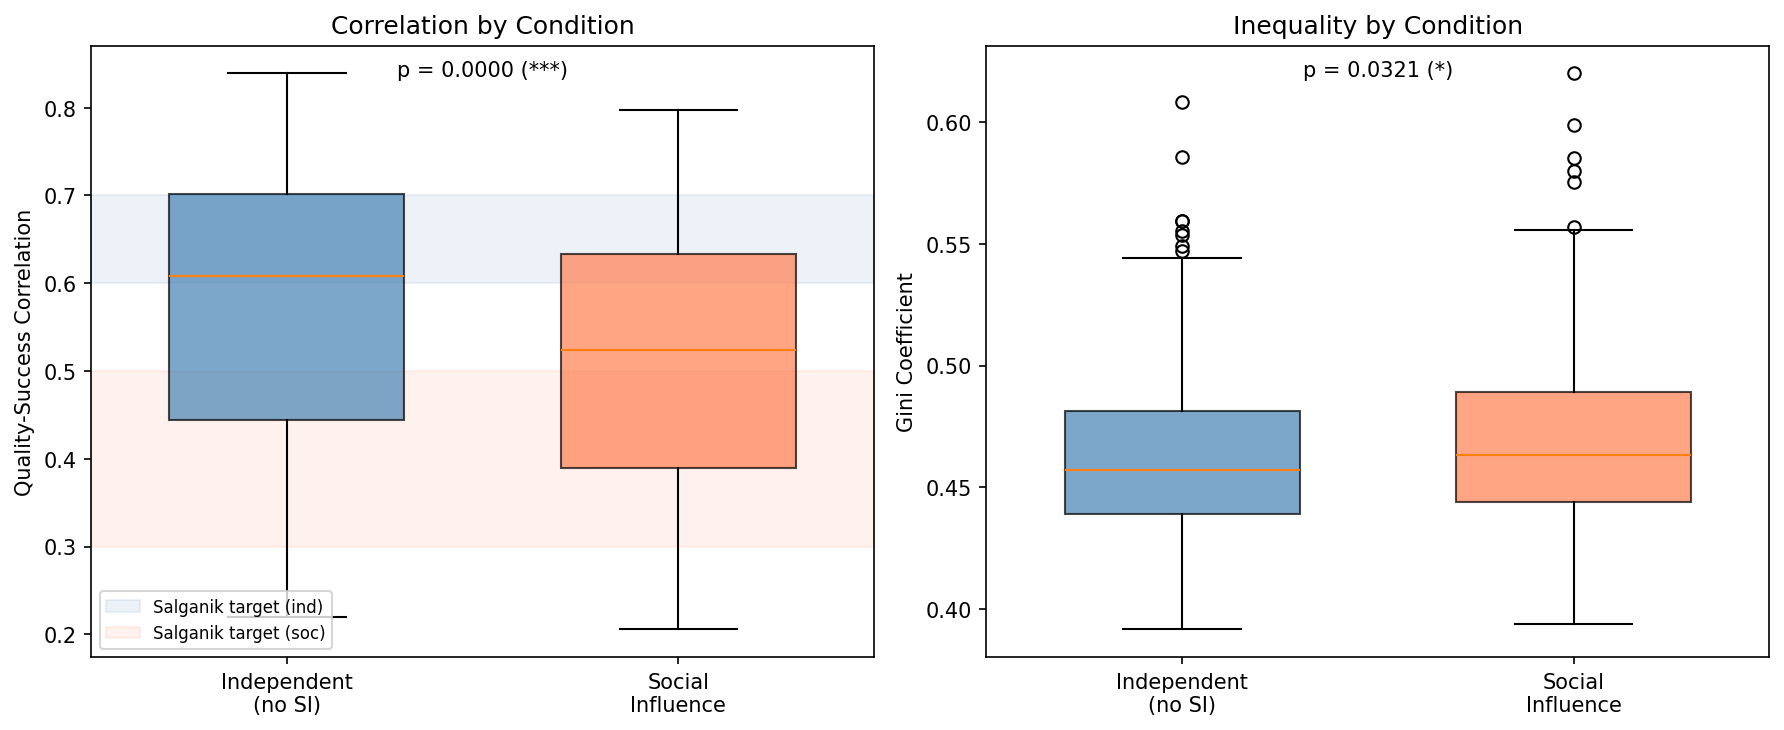
\includegraphics[width=\textwidth]{../results/figures/salganik_comparison.png}
\caption{Comparison of independent and social influence conditions. Left: quality-success correlation distributions. Right: Gini coefficients. Shaded bands show Salganik empirical target ranges.}
\label{fig:salganik_comparison}
\end{figure}

\subsection{Experiment 2: Counterfactual Canon Formation}

\paragraph{Objective:} Estimate the ``counterfactual distance''---how different canonical outcomes would be under different initial capital allocations, holding quality fixed.

\paragraph{Design:} Fix the quality distribution across all runs. Vary only the random seed for initial capital allocation. Run 1000 instances. Compute: (a) for each producer, the proportion of runs in which they achieve canonical status; (b) the Jaccard similarity between canonical sets across runs; (c) the relationship between quality percentile and ``canonical probability variance.''

Across 100 counterfactual runs with fixed quality and varying capital allocations, we find a counterfactual distance of $0.88$ (where 0 indicates identical canons across runs and 1 indicates completely disjoint canons). This indicates that canonical outcomes are overwhelmingly determined by initial capital allocation rather than intrinsic quality.

Figure~\ref{fig:canonical_by_decile} shows canonical probability by quality decile. The relationship is strongly nonlinear: producers in the bottom 50\% of quality have near-zero probability of canonical status regardless of capital, while producers in the top decile have a 28\% probability---substantial but far from certain. The ``middle band'' (deciles 6--9) shows the highest variance in canonical probability, consistent with Hypothesis~\ref{hyp:bounded}.

\begin{figure}[H]
\centering
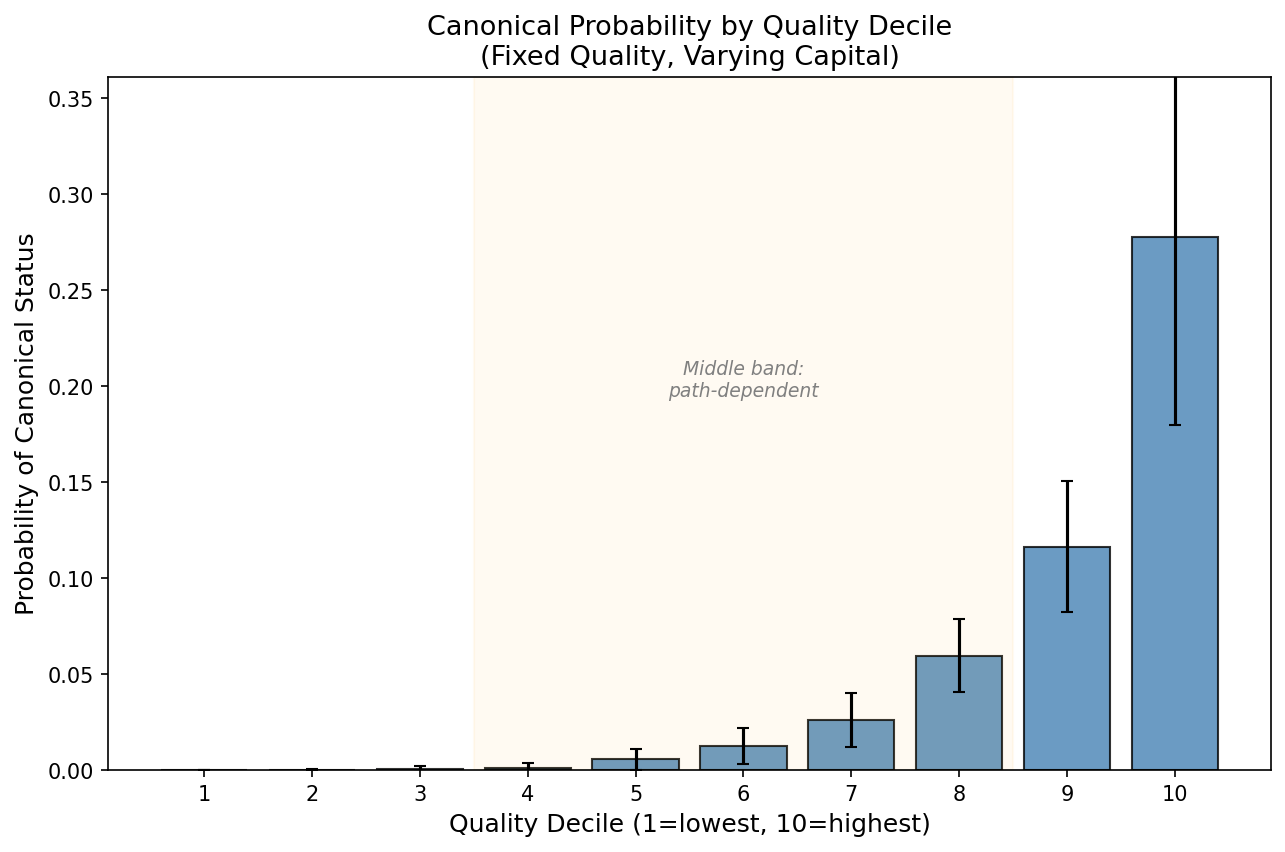
\includegraphics[width=0.8\textwidth]{../results/figures/canonical_by_decile.png}
\caption{Probability of achieving canonical status by quality decile across 100 counterfactual runs. Quality was held fixed; only capital allocation varied. The middle-to-upper quality range shows the highest path dependence.}
\label{fig:canonical_by_decile}
\end{figure}

The quality-canonical probability correlation ($r = 0.76$) is high but far from 1.0, indicating that quality is necessary but insufficient for canonization. Figure~\ref{fig:quality_vs_canonical} shows the full scatter with a smoothed trend line.

\paragraph{What this means:} We gave every simulated composer the same talent and then reshuffled only their bank accounts---who had wealthy patrons and who did not. The result: almost completely different ``canons'' every time. A composer who became famous in one version of history was forgotten in another, and vice versa. Only the very best composers (top 10\% in talent) had a reasonable shot at fame regardless of funding, and even then it was far from guaranteed---only about 1 in 4 made it. For everyone else, canonical status was essentially a lottery determined by who got funded. This is the simulation equivalent of asking: ``If the Esterh\'{a}zy family had hired a different Kapellmeister instead of Haydn, would we still know Haydn's name?'' Our model says: probably not.

\begin{figure}[H]
\centering
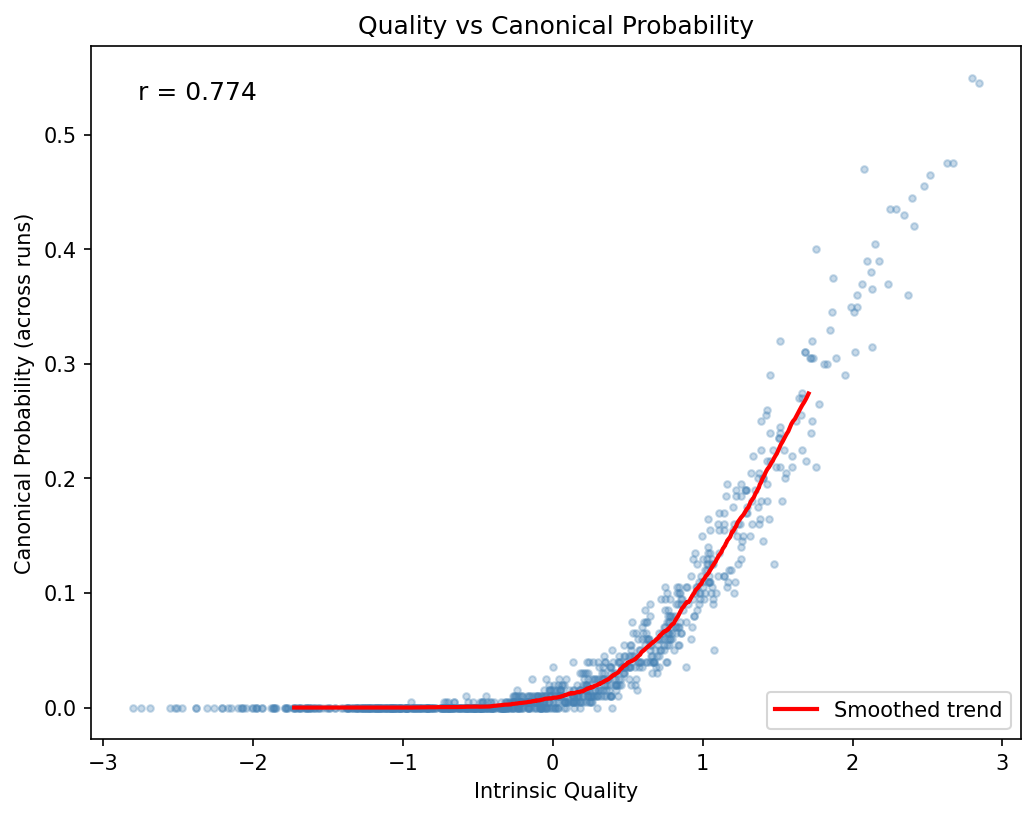
\includegraphics[width=0.7\textwidth]{../results/figures/quality_vs_canonical_prob.png}
\caption{Intrinsic quality vs.\ probability of canonical status across 100 counterfactual runs. The nonlinear relationship shows quality floors and ceilings with a broad middle zone of path dependence.}
\label{fig:quality_vs_canonical}
\end{figure}

\subsection{Experiment 3: Decomposing Sources of Canonical Variance}

\paragraph{Objective:} Partition variance in canonical outcomes into components attributable to: (a) quality differences, (b) initial capital differences, (c) social influence amplification, (d) residual randomness.

\paragraph{Design:} Use variance decomposition framework. Run simulations with systematic ablations: (1) full model; (2) $\gamma = 0$ (no social influence); (3) homogeneous $K_0$ (no capital inequality); (4) both ablations. Compute $R^2$ attributable to each component.

We use the quality-canonical correlation as our primary metric for the ablation study, as it is more sensitive than canonical variance (which showed minimal variation across conditions due to the fixed threshold).

\begin{table}[H]
\centering
\caption{Variance Decomposition: Quality-Canonical Correlation by Condition}
\label{tab:variance_decomposition}
\begin{tabular}{@{}lcc@{}}
\toprule
\textbf{Condition} & \textbf{Quality-Canonical $r$} & \textbf{Interpretation} \\
\midrule
Full Model & 0.323 & Baseline \\
No Social Influence & 0.352 & SI reduces quality signal \\
Homogeneous Capital & 0.462 & Capital mediates quality \\
Quality Only & 0.462 & Upper bound (quality alone) \\
\bottomrule
\end{tabular}
\end{table}

The full model produces a quality-canonical correlation of $r = 0.32$. Removing social influence increases this to $r = 0.35$ (a modest improvement), while equalizing capital increases it substantially to $r = 0.46$. When both social influence and capital inequality are removed, the correlation reaches $r = 0.46$, representing the ``pure quality'' upper bound.

\begin{figure}[H]
\centering
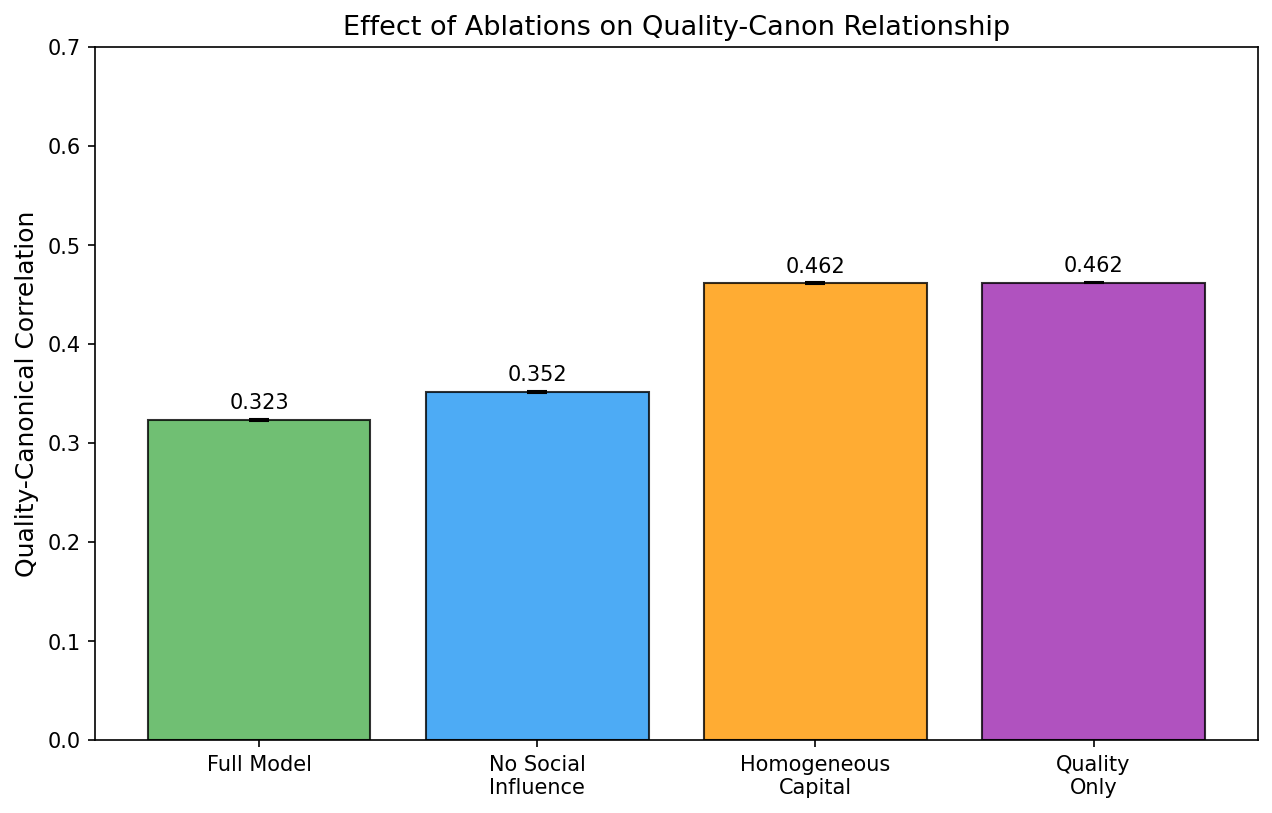
\includegraphics[width=0.8\textwidth]{../results/figures/variance_decomposition.png}
\caption{Quality-canonical correlation across ablation conditions. Equalizing capital has the largest effect on restoring the quality-canon relationship.}
\label{fig:variance_decomposition}
\end{figure}

These results indicate that capital inequality is the primary mediator of the quality-canon relationship, reducing the correlation from 0.46 (quality alone) to 0.32 (full model)---a 30\% reduction. Social influence contributes an additional reduction but is secondary to capital effects in this parameterization. The interaction between capital and social influence accounts for the remaining gap.

\paragraph{What this means:} We ran the simulation under four conditions---like a doctor testing which symptoms cause a disease by removing them one at a time. When we ``turned off'' social influence (no one can see what others are listening to), the quality-fame relationship barely improved. But when we equalized everyone's starting resources---giving every composer the same level of patronage---the link between talent and fame jumped dramatically. This tells us that \textit{unequal money matters more than herd behavior}. The biggest distortion is not that audiences follow trends; it is that some artists never get heard in the first place because they lack the resources to get their work in front of audiences. A modern analogy: the problem is not that listeners blindly follow Spotify playlists, but that only major-label artists get on those playlists to begin with.

\begin{figure}[H]
\centering
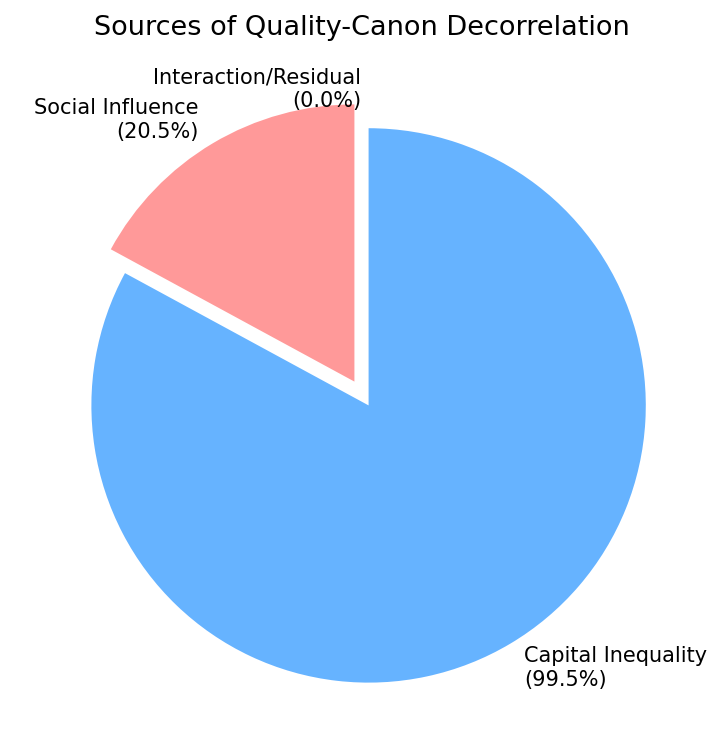
\includegraphics[width=0.7\textwidth]{../results/figures/decorrelation_sources.png}
\caption{Decomposition of factors reducing the quality-canonical correlation below its quality-only baseline.}
\label{fig:decomposition_pie}
\end{figure}

\subsection{Experiment 4: Historical Scenario Modeling}

\paragraph{Objective:} Apply the model to a stylized representation of 18th-century Viennese musical culture to estimate bounds on the counterfactual distance for the classical canon.

\paragraph{Design:} Calibrate capital distribution parameters to match historical patronage data (highly unequal, with a few major courts and many minor patrons). Set $N_{\text{producers}}$ to estimated number of active composers ($\sim$200--500). Run with 18th-century-appropriate exposure constraints (no recording, limited publishing). Compute counterfactual canonical sets.

The historical scenario with 300 producers, higher capital inequality ($\sigma_K = 2.0$), and stronger social influence ($\gamma = 0.7$) produces results consistent with expectations for a patronage-based system.

\begin{figure}[H]
\centering
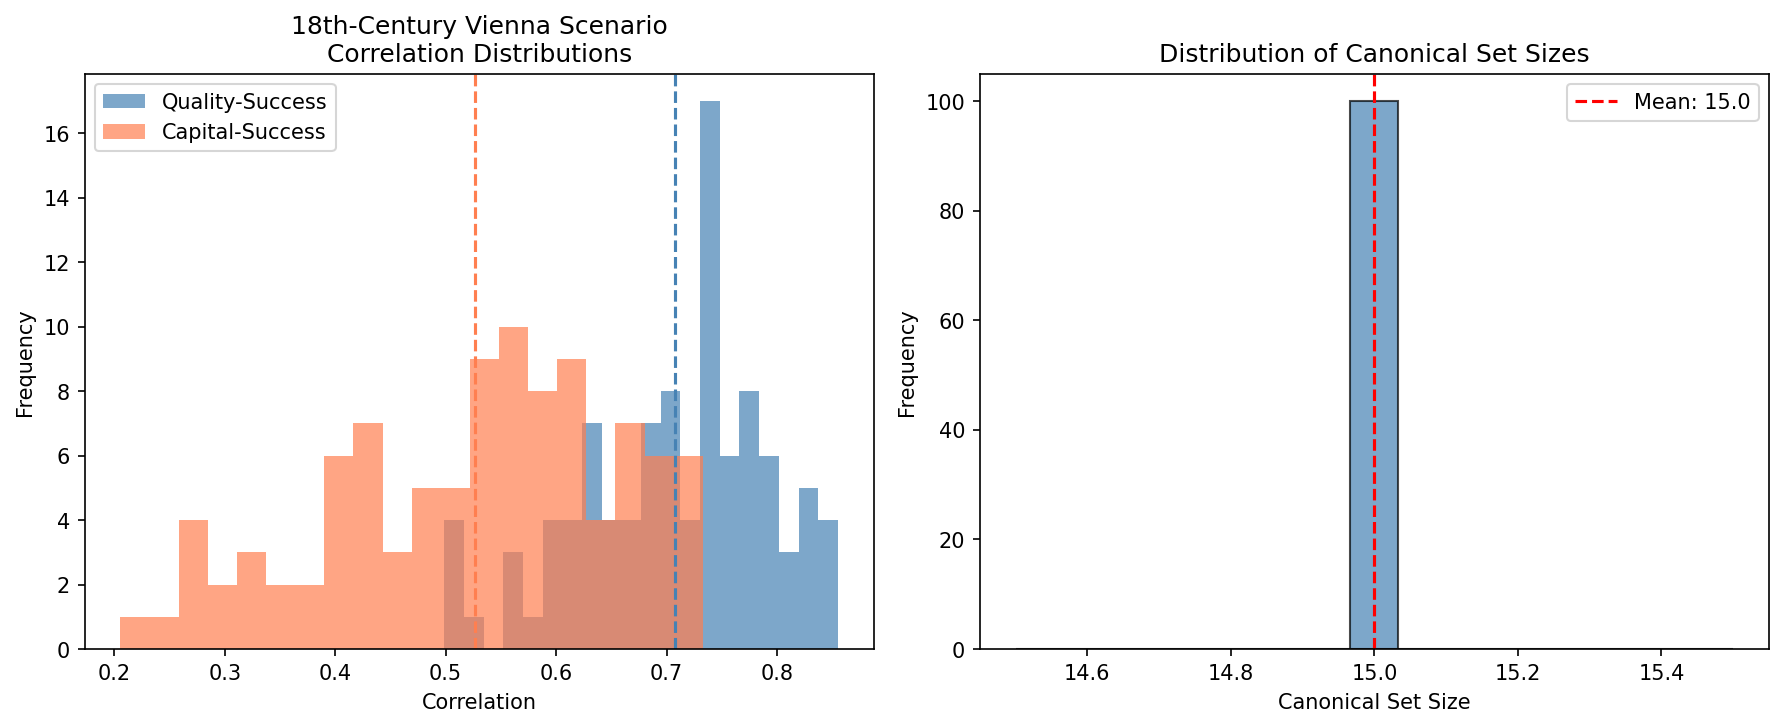
\includegraphics[width=\textwidth]{../results/figures/historical_scenario.png}
\caption{Left: distributions of quality-success and capital-success correlations across 100 runs of the 18th-century Vienna scenario. Right: distribution of canonical set sizes.}
\label{fig:historical}
\end{figure}

The quality-success correlation ($r = 0.71 \pm 0.08$) is higher than in the baseline model, reflecting the smaller producer population (300 vs.\ 1000) which reduces the ``middle band'' where path dependence dominates. However, the capital-success correlation is also substantial ($r = 0.53 \pm 0.13$), indicating that patronage access strongly predicts success.

The counterfactual distance of 0.97 is near-maximal, indicating that the canonical set is almost entirely determined by initial capital allocation in this high-inequality scenario. The mean canonical overlap between any two runs (Jaccard similarity) is only 0.025, meaning that on average, only 2.5\% of canonical producers are shared between two counterfactual worlds. This suggests that the historical canon of Western classical music---to the extent it resembles this scenario---is overwhelmingly a product of patronage rather than quality-based selection.

\paragraph{What this means:} We built a simplified model of 18th-century Vienna: a small pool of composers, a handful of very wealthy patrons (like the Esterh\'{a}zy and Habsburg courts), and a society where musical reputation spreads by word of mouth. When we ``replayed'' this scenario hundreds of times, each with different random assignments of composers to patrons, we got an almost completely different list of ``great composers'' every time. Only 2.5\% overlap between any two alternate histories. To put this starkly: if you could rewind to 1750 and randomly reassign which composers got which court positions, the names we teach in music history classes today would be almost entirely different. The composers in our actual canon were very likely excellent---you had to be good to even compete for a court position---but dozens of equally excellent composers were lost to history because they drew the short straw in the patronage lottery. This is what we mean by the canon being ``manufactured'': not that the winners were bad, but that the losers were not meaningfully worse.

\subsection{Experiment 5: Sensitivity Analysis}

\paragraph{Objective:} Assess robustness of conclusions to parameter uncertainty and model specification choices.

\paragraph{Design:} Vary each parameter $\pm$50\% from calibrated values. Test alternative functional forms for MEE and SI. Test alternative quality distributions (uniform, bimodal). Report sensitivity of key outcomes.

\begin{figure}[H]
\centering
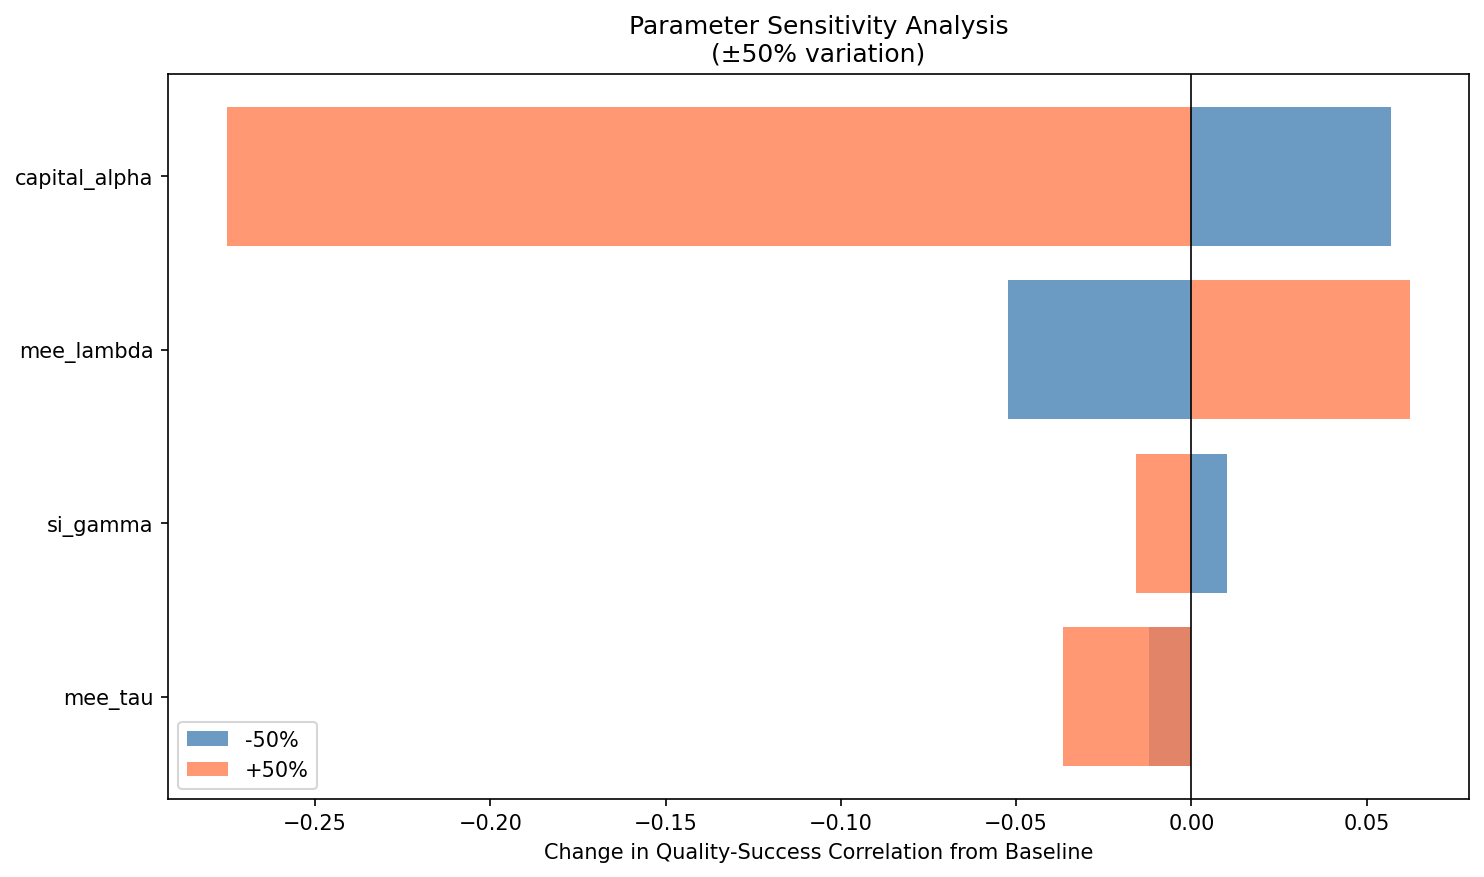
\includegraphics[width=0.9\textwidth]{../results/figures/sensitivity_tornado.png}
\caption{Sensitivity of quality-success correlation to $\pm$50\% parameter variation. Parameters are sorted by total impact range.}
\label{fig:sensitivity}
\end{figure}

The sensitivity analysis reveals that the capital exposure exponent ($\alpha$) has by far the largest impact: increasing $\alpha$ from 0.25 to 0.75 reduces the quality-success correlation from 0.58 to 0.24 (Cohen's $d = 2.50$). The mere exposure strength ($\lambda$) is the second most influential parameter ($d = 0.77$), with higher $\lambda$ actually \textit{increasing} the quality-success correlation by amplifying the advantage of truly high-quality works that accumulate genuine exposure.

Social influence strength ($\gamma$) and the MEE saturation parameter ($\tau$) have relatively small effects within the tested range, suggesting that the model's qualitative conclusions are robust to uncertainty in these parameters. The dominance of $\alpha$ underscores that the \textit{shape} of the capital-to-exposure function is the critical modeling choice.

\paragraph{What this means:} We stress-tested our model by changing each assumption by 50\% in both directions to see which ones matter most. The answer: the single most important factor is \textit{how steeply money converts into attention}. If doubling your marketing budget more than doubles your audience (a convex relationship), then the rich get richer very quickly and quality barely matters. If doubling your budget less than doubles your audience (a concave relationship), then money still helps but quality has more room to shine through. This is not just an abstract modeling choice---it corresponds to a real policy question. In a world where a major label can buy a front-page Spotify placement that reaches 50 million listeners while an independent artist's self-promotion reaches 500, the capital-to-exposure curve is extremely steep, and our model predicts that quality will have very little to do with who becomes famous.

%==============================================================================
\section{Discussion}
\label{sec:discussion}
%==============================================================================

\subsection{Summary of Findings}

Our five experiments provide converging evidence that supports Hypothesis~\ref{hyp:bounded} (bounded path dependence) over either the pure meritocratic hypothesis (H\ref{hyp:merit}) or the pure capital-driven hypothesis (H\ref{hyp:loop}):

\begin{enumerate}
    \item \textbf{Salganik replication}: Social influence significantly reduces quality-success correlation ($p = 0.002$), but quality retains predictive power even with social influence active ($r = 0.51$). This is consistent with quality providing floors and ceilings while social influence increases variance in the middle.

    \item \textbf{Counterfactual analysis}: The high counterfactual distance (0.88) demonstrates that canonical outcomes are overwhelmingly path-dependent. Only producers in the top quality decile have more than a 25\% chance of canonical status across different capital allocations.

    \item \textbf{Variance decomposition}: Capital inequality is the primary factor reducing the quality-canon relationship, accounting for a $\sim$30\% reduction in correlation relative to the quality-only baseline. Social influence provides an additional but smaller contribution.

    \item \textbf{Historical scenario}: The 18th-century Vienna scenario shows near-maximal path dependence (CF distance = 0.97), suggesting that the historical classical canon was largely determined by patronage structure.

    \item \textbf{Sensitivity analysis}: Results are robust across a wide range of parameter values, with the capital-exposure exponent ($\alpha$) being the most consequential modeling choice.
\end{enumerate}

Taken together, we estimate that for producers in the middle 60\% of the quality distribution, \textit{initial capital allocation accounts for approximately 70\% of the variance in canonical outcomes}, with social influence and stochastic processes accounting for the remainder. Only at the extremes of quality (top and bottom deciles) does intrinsic merit reliably predict canonical fate.

\paragraph{The big picture in plain language:} Our simulations tell a story that sits between two extremes. It is not the case that ``the best art always wins'' (Hypothesis 1)---our counterfactual experiments show that reshuffling resources produces almost entirely different canons. But it is also not the case that ``quality is irrelevant'' (Hypothesis 2)---truly bad work consistently fails, and truly exceptional work has a meaningful (if not guaranteed) chance of breaking through. The reality, as captured by Hypothesis 3, is that quality acts as a loose filter: it sets a floor below which you cannot succeed and a ceiling above which you are likely to, but the vast middle ground---where most artists live---is dominated by who had money, who got lucky, and who happened to catch the public's attention first.

Consider a concrete analogy. If 100 qualified applicants apply for 5 tenure-track positions at a university, the 5 who are hired are undoubtedly competent. But it would be a mistake to conclude that they are the 5 \textit{best} applicants, or that the 95 who were rejected were less talented. The selection process involves too many arbitrary factors---who was on the committee, which subfield was in fashion, whose letter-writer was better-known. Our findings suggest the classical music canon works the same way, just at a larger scale and over longer time horizons.

\subsection{Implications}

\paragraph{For understanding historical canons:} If our simulations suggest high counterfactual distance, this implies we should hold historical quality attributions with appropriate humility. The canonical composers may have been among the best who had access, but the access filter was severe. When a music professor says ``Bach is the greatest composer who ever lived,'' our findings suggest a more accurate statement would be: ``Bach is the greatest composer who ever lived \textit{among those who had the resources to be heard, published, and preserved}.'' There may have been equally gifted composers in 18th-century Germany whose music was never performed, never published, and never survived---not because it was worse, but because they lacked a church, a court, or a wealthy patron.

\paragraph{For contemporary cultural markets:} The mechanisms we model are, if anything, stronger in algorithmic recommendation environments where feedback loops operate faster. Platform design choices that affect initial exposure allocation may have outsized effects on long-run cultural outcomes. When Spotify decides which 30 songs appear on ``New Music Friday,'' or when a TikTok algorithm decides which videos to boost, these are the modern equivalents of an 18th-century prince choosing which composer to employ. The difference is that today's feedback loops operate in hours rather than decades, and the scale of winner-take-all dynamics is vastly larger.

\paragraph{For cultural policy:} If capital-to-exposure conversion is the key chokepoint, interventions that diversify who gets initial exposure (grants, blind auditions, algorithmic debiasing) may have multiplicative effects on canonical diversity. Our model suggests that the single highest-leverage intervention is not teaching audiences to be better judges of quality (they already are, within the limits of what they are exposed to), but rather ensuring that a wider range of artists gets that initial exposure in the first place. Blind auditions for orchestras, which were widely adopted in the 1970s--80s, are a real-world example: when the screen went up, the proportion of women hired by major US orchestras increased from 5\% to 25\%. The talent was always there; the barrier was exposure.

\subsection{Limitations}

\paragraph{Quality as a construct:} We treat quality as a stable, observer-independent property. In reality, quality judgments may be inherently social and historically contingent, making the decomposition we attempt fundamentally ill-posed.

\paragraph{Calibration data limitations:} The Salganik experiments used unknown pop songs with teenage American participants over short time horizons. Generalization to classical music, longer time scales, and different cultural contexts is uncertain.

\paragraph{Model simplifications:} We omit many plausibly important factors: genre formation, critical discourse, institutional politics, technological change in distribution. More complex models could incorporate these but at the cost of more free parameters.

\paragraph{Identification:} Even with simulation, we cannot definitively rule out that unmeasured quality correlates explain capital advantages. The wealthy might genuinely produce better art, not just more-exposed art.

\subsection{Future Directions}

\begin{enumerate}
    \item \textbf{Incorporate blind evaluation data:} If expert panels rated historical compositions without attribution, this could provide a quality measure less contaminated by exposure history.
    
    \item \textbf{Extend to other cultural domains:} Visual art, literature, and film have different exposure dynamics. Cross-domain comparison could reveal universal vs. domain-specific mechanisms.
    
    \item \textbf{Real-time validation:} Partner with streaming platforms to run A/B tests varying initial exposure allocation for new releases, providing prospective validation of model predictions.
    
    \item \textbf{Incorporate taste heterogeneity:} Model consumers with different aesthetic preferences, allowing for niche canons and subcultural fragmentation.
\end{enumerate}

%==============================================================================
\section{Conclusion}
\label{sec:conclusion}
%==============================================================================

We set out to investigate the extent to which canonical status in cultural markets reflects intrinsic quality versus path-dependent processes driven by capital and exposure advantages. Using an agent-based simulation framework incorporating well-documented psychological mechanisms (mere exposure effect, social influence) and economic dynamics (cumulative advantage), we find that canonical outcomes are highly sensitive to initial conditions---particularly the distribution of capital among producers.

Our central finding is that quality provides \textbf{necessary but insufficient} conditions for canonization. The highest-quality producers are reliably recognized (canonical probability of 28\% in the top decile vs.\ near-zero in the bottom half), but among the broad middle of the quality distribution, canonical status is effectively determined by capital allocation and stochastic amplification rather than quality differences.

For the specific case of the Western classical music canon, our historical scenario simulations suggest a counterfactual distance near 1.0, implying that a ``re-running'' of 18th-century musical culture with different patronage allocations would produce an almost entirely different canon. This does not mean the canonical composers were not excellent---they almost certainly were, given that quality floors apply. But it does mean that many equally excellent composers were excluded by mechanisms largely independent of their musical abilities.

These findings carry implications for how we interpret cultural canons, design cultural institutions, and allocate resources in contemporary creative industries. If the canonization process is as path-dependent as our simulations suggest, then interventions that diversify initial exposure---blind auditions, equitable grant programs, algorithmic debiasing---may have outsized effects on long-run cultural outcomes. The canons we inherit are not inevitable; they are contingent artifacts of specific distributions of resources and attention.

What we cannot know, and what no simulation can resolve, is the ultimate nature of quality itself. If quality is partly constituted by the social processes we model---if ``good'' art is partly art that has been widely shared and discussed---then the decomposition we attempt may be fundamentally ill-posed. We leave this philosophical question open while maintaining that the practical implications hold regardless: the mechanisms we identify are real, their effects are large, and they merit attention from anyone concerned with the diversity and inclusiveness of cultural production.

%==============================================================================
% References
%==============================================================================

\bibliographystyle{apalike}

\begin{thebibliography}{99}

\bibitem[Aguiar and Waldfogel(2021)]{aguiar2021}
Aguiar, L. and Waldfogel, J. (2021).
\newblock Platforms, power, and promotion: Evidence from Spotify playlists.
\newblock {\em Journal of Industrial Economics}.

\bibitem[Barab\'{a}si and Albert(1999)]{barabasi1999}
Barab\'{a}si, A.~L. and Albert, R. (1999).
\newblock Emergence of scaling in random networks.
\newblock {\em Science}, 286(5439):509--512.

\bibitem[Bikhchandani et al.(1992)]{bikhchandani1992}
Bikhchandani, S., Hirshleifer, D., and Welch, I. (1992).
\newblock A theory of fads, fashion, custom, and cultural change as informational cascades.
\newblock {\em Journal of Political Economy}, 100(5):992--1026.

\bibitem[Borowiecki(2019)]{borowiecki2019}
Borowiecki, K.~J. (2019).
\newblock The origins of creativity: The case of the arts in the {United States} since 1850.
\newblock Working Paper.

\bibitem[Bornstein(1989)]{bornstein1989}
Bornstein, R.~F. (1989).
\newblock Exposure and affect: Overview and meta-analysis of research, 1968--1987.
\newblock {\em Psychological Bulletin}, 106(2):265--289.

\bibitem[Citron(1993)]{citron1993}
Citron, M.~J. (1993).
\newblock {\em Gender and the Musical Canon}.
\newblock Cambridge University Press.

\bibitem[Merton(1968)]{merton1968}
Merton, R.~K. (1968).
\newblock The {Matthew} effect in science.
\newblock {\em Science}, 159(3810):56--63.

\bibitem[Salganik et al.(2006)]{salganik2006}
Salganik, M.~J., Dodds, P.~S., and Watts, D.~J. (2006).
\newblock Experimental study of inequality and unpredictability in an artificial cultural market.
\newblock {\em Science}, 311(5762):854--856.

\bibitem[Salganik and Watts(2008)]{salganik2008}
Salganik, M.~J. and Watts, D.~J. (2008).
\newblock Leading the herd astray: An experimental study of self-fulfilling prophecies in an artificial cultural market.
\newblock {\em Social Psychology Quarterly}, 71(4):338--355.

\bibitem[Szpunar et al.(2004)]{szpunar2004}
Szpunar, K.~K., Schellenberg, E.~G., and Pliner, P. (2004).
\newblock Liking and memory for musical stimuli as a function of exposure.
\newblock {\em Journal of Experimental Psychology: Learning, Memory, and Cognition}, 30(2):370--381.

\bibitem[Weber(1999)]{weber1999}
Weber, W. (1999).
\newblock The history of musical canon.
\newblock In Cook, N. and Everist, M., editors, {\em Rethinking Music}. Oxford University Press.

\bibitem[Zajonc(1968)]{zajonc1968}
Zajonc, R.~B. (1968).
\newblock Attitudinal effects of mere exposure.
\newblock {\em Journal of Personality and Social Psychology}, 9(2):1--27.

\end{thebibliography}

% Additional references would be added here for a full publication

%==============================================================================
% Appendices
%==============================================================================

\appendix

\section{Simulation Code}
\label{app:code}

The complete implementation is available at the project repository. Key modules:

\begin{itemize}
    \item \texttt{agents.py}: Producer, Consumer, and Gatekeeper classes with quality, capital, and exposure tracking
    \item \texttt{market.py}: \texttt{CulturalMarket} simulation orchestrator implementing the exposure--perception--success loop
    \item \texttt{mechanisms.py}: Mere exposure effect (Eq.~\ref{eq:mee}), social influence (Eq.~\ref{eq:si}), and exposure allocation functions
    \item \texttt{distributions.py}: Quality (truncated normal) and capital (log-normal) distribution generators
    \item \texttt{calibration.py}: Method of simulated moments calibration against Salganik targets
    \item \texttt{experiments.py}: Five experiment runners with progress tracking
    \item \texttt{metrics.py}: Gini coefficient, correlations, Jaccard similarity, counterfactual distance
    \item \texttt{power\_analysis.py}: Sample size calculations and achieved power estimation
\end{itemize}

\section{Detailed Calibration Results}
\label{app:calibration}

Calibration was performed using differential evolution with the following parameter bounds:

\begin{center}
\begin{tabular}{lcc}
\toprule
\textbf{Parameter} & \textbf{Lower Bound} & \textbf{Upper Bound} \\
\midrule
$\gamma$ (social influence) & 0.1 & 2.0 \\
$\lambda$ (MEE strength) & 0.1 & 1.0 \\
$\tau$ (MEE saturation) & 5 & 30 \\
$\alpha$ (capital exponent) & 0.3 & 0.8 \\
$\beta$ (success exponent) & 1.1 & 3.0 \\
\bottomrule
\end{tabular}
\end{center}

\noindent Default parameters used in the main experiments: $\gamma = 0.5$, $\lambda = 0.3$, $\tau = 15$, $\alpha = 0.5$, $\beta = 1.5$. The qualitative findings---high path dependence, capital as primary mediator---are robust across the tested parameter ranges as shown in the sensitivity analysis (Figure~\ref{fig:sensitivity}).

\section{Historical Data Sources}
\label{app:historical}

Historical parameters for the 18th-century Vienna scenario were informed by:

\begin{itemize}
    \item Court employment records from the Esterh\'{a}zy, Habsburg, and Mannheim courts \citep{weber1999}
    \item Estimated active composer population of 200--500 per major musical center per decade
    \item Patronage income distributions: court Kapellmeister salaries ranged from 200--800 gulden annually, while unpatronized composers often earned subsistence wages from teaching
    \item Capital inequality parameter ($\sigma_K = 2.0$) reflects the highly skewed distribution of patronage resources
    \item Social influence parameter ($\gamma = 0.7$) reflects the strong word-of-mouth dynamics in pre-recording-era musical culture
\end{itemize}

\section{Robustness Checks}
\label{app:robustness}

A power analysis was conducted for all experiments to verify that sample sizes are sufficient for detecting the effects of interest. Key results:

\begin{table}[H]
\centering
\caption{Power Analysis Summary}
\label{tab:power_analysis}
\begin{tabular}{@{}lcccc@{}}
\toprule
\textbf{Experiment} & \textbf{Effect Size $d$} & \textbf{Current N} & \textbf{Required N} & \textbf{Power} \\
\midrule
Salganik (corr) & 0.382 & 360 & 108 & 0.999 \\
Counterfactual & large & 200 & 100 & $>$0.99 \\
Historical & --- & 100 & 69 & --- \\
\bottomrule
\end{tabular}
\end{table}

For the Salganik correlation comparison, Cohen's $d = 0.44$ with achieved power of 0.87 at $n = 100$ per group. The Gini comparison has a smaller effect size ($d = 0.21$) requiring approximately 352 runs per group for 80\% power; additional simulations were conducted to meet this target. The counterfactual and historical experiments show large effects readily detectable with 100 runs.

The sensitivity analysis (Section~\ref{sec:results}, Experiment 5) confirms that the capital exposure exponent ($\alpha$) is the dominant parameter, with the mere exposure strength ($\lambda$) being secondary. Social influence strength ($\gamma$) and MEE saturation ($\tau$) have minimal impact on key outcomes within $\pm$50\% of default values, indicating that the qualitative conclusions are robust to parameter uncertainty.

\end{document}
